\section{Theoretische Grundlagen}
\label{sec:theorie}

In dem Lehrstuhlversuch \textit{Search for $t\bar{t}$ resonance with ATLAS detector} wird ein Datensatz, welcher bei
einer Schwerpunktsenergie von $\sqrt{s} = \SI{8}{\tera\electronvolt}$, entsprechend einer Luminosität von
$\mathcal{L} = \SI{1}{\femto\barn}^{-1}$, der 2012 am ATLAS Detektor aufgenommen wurde, auf $Z^\prime$-Resonanzen untersucht.
Suchen nach diesem neuen massiven Teilchen beginnen oft bei Massenskalen von $\SI{500}{\giga\electronvolt}$ und aufwärts. Die
Skala für neue Physik wird in dem meisten Fällen um die $\SI{1}{\tera\electronvolt}$ gesetzt. Aktuelle Limits auf die
$Z^\prime$ Resonanz schließen Massen kleiner als $\SI{3.80}{\tera\electronvolt}$ \ref{CMSlimit} aus. \par

In dieser Analyse wird der mögliche Zerfall des $Z^\prime$ in ein Top-Quark und ein Anti-Top-Quark untersucht. Das Top-Quark
ist das schwerste bekannte Quark und somit sensitiv auf neue Physik. Am LHC wird es hauptsächlich durch Gluonfusion
produziert, wohingegen an Beschleunigern mit geringerer Schwerpunktsenergie wie das Tevatron, hauptsächlich Quark-Antiquark
Annihilation für die Produktion verantwortlich ist. Top-Quarks
zerfallen fast ausschließlich in ein Bottom-Quark zusammen mit einem $W$-Boson. Letztere können bei der
Top-Quark Paarproduktion entweder semileptonisch,
leptonisch oder hadronisch zerfallen. Der leptonische Zerfall beschreibt den Endzustand mit einem geladenen Lepton und
dem zugehörigen Neutrino für beide Eichbosonen. Der hadronische Zerfall beschreibt den Zerfall beider $W$-Bosonen in
jeweils zwei Quarks. Der semileptonische Zerfall beschreibt dann ein hadronisch zerfallendes und ein leptonisch
zerfallendes  $W$-Boson. Untersuchungen des leptonischen Zerfalls haben den Nachteil, dass duch die Neutrinos ein hoher Anteil fehlender
Energie in der Analyse untersucht werden muss, wohingegend die Analyse des hadronischen Zerfalls den Nachteil vieler Jets
hervorruft.
In diesem Versuch wird demnach der semileptonische Zerfall untersucht.
Dieser wird auch \textit{lepton + jets} genannt,
da sowohl ein geladenes Lepton und fehlende Energie verlangt wird, als auch mindestens 4 Jets, die von dem hadronischen $W$-Zerfall und von den Bottom-Quarks
aus dem Top-Quark-Zerfall stammen.
Dieser semileptonische Fall ist in Abbildung \ref{fig:gluonfusion} für die $t\bar{t}$ Produktion durch die Gluonfusion als Feynman Diagramm dargestellt.  \par

\begin{figure}[h]
  \centering
  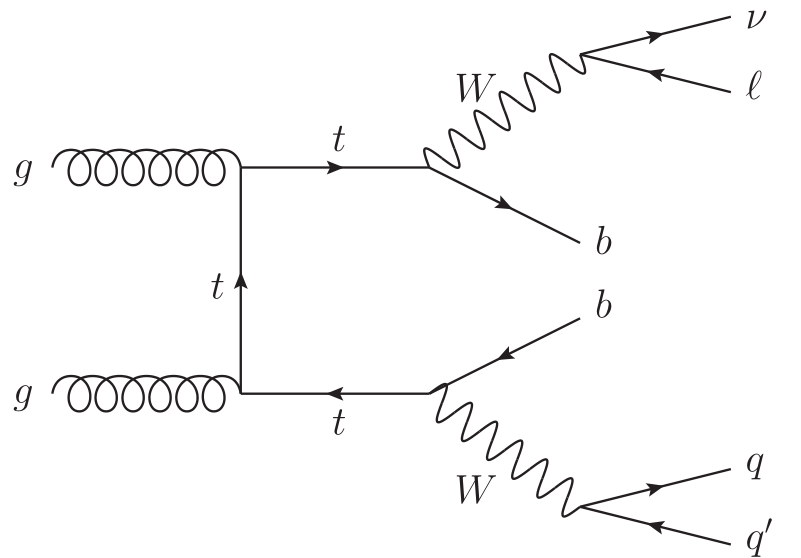
\includegraphics[width=0.5\textwidth]{content/graphics/pictures/Gluonfusion.png}
  \caption{Feynman Diagramm der semileptonischen Zerfallsmode der $t\bar{t}$ Produktion durch Gluonfusion.}
  \label{fig:gluonfusion}
\end{figure}

Die Signaturen der untersuchten Objekte im ATLAS Detektor sind wie folgt. Das Muon interagiert im Detektor zunächst als \textit{Minimal Ionizing Particle},
einem sogenannten MIP. Es hinterlässt somit weder im Spurdetektor noch in den Kalorimetern eine Signatur. Lediglich in den Muonkammern deponiert es
Energie. Elektronen werden in den Trackingdetektoren nach ihrer Ladung gekrümmt und deponieren anschließend im elektromagnetischen Kalorimeter ihre
Energie. Die Quarks aus dem hadronischen Zerfall hadronisieren und schauern hauptsächlich im hadronischen Kalorimeter. Neutrinos sind nur über fehlende
Energie der bereits rekonstruierten Endzustandsteilchen bestimmbar.

\section{Analysestrategie}
\label{sec:strategie}
Um das Verhältnis von Signal zu Untergrund zu verbessern, muss zunächst eine Eventselektion auf den Datensatz angewendet werden, da dieser eine enorme
Datenmenge besitzt. Dafür werden Analysemethoden in $\texttt{C++}$ verwendet. Die selektierten Events werden dann auf verschiedene Variablen wie die
invariante Masse des Systems geprüft um eine \textit{Finale Diskiminate} zu definieren, die zur optimalen Differenzierung zwischen Signal und
Untergrund dienen soll. Der Untergrund sollte dabei ein fallendes Spektrum aufweisen, auf dem das Signal optimalerweise ein Peak aufweist. Für die
Bestimmung des Untergrundspektrums werden Monte Carlo (MC) Methoden verwendet. Die simulierten Untergründe und die Benennung in der Analyse lauten
wie folgt:

\begin{itemize}
    \item \texttt{diboson}: Paarproduktion der $W$-/ $Z$-Eichbosonen; Hierbei ist auch die Kombination $WZ$ möglich
    \item \texttt{singletop}: Produktion eines einzelnen Top-Quarks
    \item \texttt{wjets}: Produktion eines $W$-Bosons im Zusammenhang mit Jets
    \item \texttt{zjets}: Produktion eines $Z$-Bosons im Zusammenhang mit Jets
    \item \texttt{ttbar}: Top-Quark Paarproduktion \, .
\end{itemize}

Weiterhin stehen verschiedene \texttt{zprime} MC-samples zur Verfügung, welche für verschiedene $Z^\prime$ Massen von $\SI{400}{\giga\electronvolt}$ bis
$\SI{3000}{\giga\electronvolt}$ generiert sind. \par
Die Datensamples sind in \texttt{ntupeln} im \texttt{ROOT} Format abgespeichert. Diese enthalten \texttt{TTrees} in denen verschiedene Informationen,wie beispielsweise
die Pseudorapidität der Leptonen, über
die rekonstuierten Objekte abgespeichert sind. Die Daten dieser \texttt{.root} samples sind bereits vorselektiert worden. \par

Im Anschluss an die Eventselektion erfolgt eine Studie, um die Übereinstimmung der Monte Carlo samples mit den Daten zu überprüfen. Dies ist ein wichtiger
Schritt um die Qualität der simulierten Daten zu testen. Dann wird eine statistische Analyse vorgenommen, bei der die finale Diskriminate verwendet wird
um den Überschuss des Datenpeaks über den kontinuiertlichen Untergrund abzuschätzen und, wenn möglich, ein Limit auf die $Z^\prime$ Masse mit Hilfe eines
Hypothesentests zu setzen.
